\chapter{Osilator Mekanik: Peredaman dan Resonansi}\label{ch:b1:oscillators-resonance}

Doronglah ayunan seorang anak pada saat yang keliru dan tak banyak yang
terjadi; doronglah sekali tiap periode, dengan lembut, dan dalam belasan
ayunan anak itu sudah menjerit di puncak busurnya. Sebuah mesin cuci
bergetar hebat pada satu laju tertentu dalam putaran perasnya lalu
tenang di atasnya. Sebuah gelas anggur bernyanyi ketika jari basah
mengelilingi bibirnya dengan laju yang tepat, dan pecah ketika seorang
penyanyi menahan nada yang sama cukup keras. Setiap peristiwa itu adalah
sebuah \emph{resonansi}: sistem yang mempunyai \omterm{def:b1:oscillators-resonance:harmonic}{frekuensi alami}, ketika
digerakkan di dekat frekuensi itu, menghimpun energi daur demi daur
sampai gesekannya menguras energi itu secepat masuknya. Bab ini
mengambil osilator mekanik --- bebas, teredam, lalu dipaksa --- dan
menurunkan kurva resonansi yang kembaran listriknya telah muncul dalam
\cref{ch:b1:sinusoidal-impedance}.

\section{Osilator harmonik}

\begin{definition}[Osilator harmonik]\label{def:b1:oscillators-resonance:harmonic}
\index{osilator harmonik}\index{frekuensi alami}
Sistem yang simpangannya $x$ dari sebuah kesetimbangan mantap menuruti
\[
\ddot x + \omega_0^2\,x = 0
\]
disebut \emph{osilator harmonik} dengan \emph{\omterm{def:b1:transient-regimes:secondorder}{frekuensi sudut alami}}
$\omega_0$ (berperiode $T_0 = 2\pi/\omega_0$). Penyelesaiannya $x = A\cos(\omega_0t
+ \varphi)$ mempunyai \omterm{def:b1:wave-propagation:signal}{amplitudo} dan fase yang ditetapkan syarat awalnya
serta periode yang bebas dari \omterm{def:b1:wave-propagation:signal}{amplitudonya} (\emph{keisokronan}).
\end{definition}

\begin{proposition}[Dari mana osilator harmonik berasal]\label{prop:b1:oscillators-resonance:sources}
\begin{itemize}
  \item Massa $m$ pada pegas $k$: $\omega_0^2 = k/m$ (\omterm{prop:b1:newton-dynamics:springstring}{hukum Hooke}).
  \item \omterm{ex:b1:newton-dynamics:pendulum}{Bandul sederhana} sepanjang $\ell$, sudut kecil: $\omega_0^2 = g/\ell$.
  \item Sebarang partikel di dekat kesetimbangan mantap sebuah potensial
        $E_p$: $\omega_0^2 = E_p''(x_0)/m$
        (\cref{prop:b1:work-and-energy:stability}).
  \item Rangkaian LC: $\omega_0^2 = 1/LC$, dengan $q \leftrightarrow x$,
        $L \leftrightarrow m$, $1/C \leftrightarrow k$.
\end{itemize}
Energinya $E = \tfrac12 m\dot x^2 + \tfrac12 m\omega_0^2x^2 = \tfrac12
m\omega_0^2A^2$ bersifat tetap, berpindah bolak-balik antara bentuk
kinetik dan bentuk potensial dua kali tiap periode.
\end{proposition}

\begin{proof}
Hukum kedua Newton dengan $F = -kx$; persamaan bandul
$\ddot\theta + (g/\ell)\sin\theta = 0$ dengan $\sin\theta \approx \theta$;
rumus Taylor di minimum $E_p$; \omterm{thm:b1:dc-circuits:kirchhoff}{hukum loop} rangkaian LC. Energinya:
turunkan lalu pakai persamaannya.
\end{proof}

\begin{example}[Silinder yang terapung-apung]\label{ex:b1:oscillators-resonance:bob}
Sebuah silinder tegak berpenampang $S$ terapung dengan kedalaman
tercelup $h$ ($mg = \rho_wgSh$, gaya apung dari
\cref{ch:b1:fluid-statics}). Ketika ditekan turun sejauh $x$, ia
menerima tambahan gaya ke atas $\rho_wgSx$: $m\ddot x = -\rho_wgSx$,
sehingga $\omega_0^2 = \rho_wgS/m = g/h$ --- sama seperti bandul
sepanjang $h$. Sebuah pelampung yang tercelup \qty{1}{m} terapung-apung
dengan periode \qty{2}{s}, berapa pun massanya.
\end{example}

\section{Osilator teredam}

\begin{proposition}[Osilator teredam]\label{prop:b1:oscillators-resonance:damped}
\index{osilator teredam}\index{faktor kualitas!mekanik}
Dengan gesekan kental $-\alpha\dot x$, persamaannya menjadi
\[
\ddot x + \frac{\omega_0}{Q}\dot x + \omega_0^2x = 0, \qquad
Q = \frac{\sqrt{km}}{\alpha} = \frac{m\omega_0}{\alpha},
\]
yaitu bentuk baku orde kedua \cref{ch:b1:transient-regimes}: untuk
$Q > \tfrac12$ sebuah peluruhan pseudoperiodik $x = A\eu^{-t/\tau}\cos(\omega t +
\varphi)$ dengan $\tau = 2Q/\omega_0$, $\omega = \omega_0\sqrt{1 - 1/4Q^2}$;
energinya meluruh sebagai $\eu^{-2t/\tau}$ dan
\[
Q = 2\pi\,\frac{\text{energi tersimpan}}{\text{energi hilang tiap periode}}
\quad (Q \gg 1) .
\]
\end{proposition}

\begin{proof}
Bagi $m\ddot x + \alpha\dot x + kx = 0$ dengan $m$. Untuk energinya: $E
\propto A^2\eu^{-2t/\tau}$ kehilangan bagian $2T/\tau = 2\pi/Q$ tiap
periode ketika nilai itu kecil.
\end{proof}

\begin{example}[Waktu berdering]\label{ex:b1:oscillators-resonance:ringing}
Sebuah garpu tala \qty{440}{Hz} masih berbunyi sepuluh sekon setelah
dipukul: \omterm{def:b1:wave-propagation:signal}{amplitudonya} jatuh ke sekitar $5\%$ dalam $3\tau = \qty{10}{s}$,
sehingga $\tau = \qty{3.3}{s}$ dan $Q = \omega_0\tau/2 \approx 4600$.
Suspensi sebuah mobil ($Q \approx 0.7$) berhenti dalam satu periode;
ayunan seorang anak ($Q \approx 20$) kehilangan sepertiga energinya tiap
ayunan dan menuntut dorongan setiap kali.
\end{example}

\section{Osilasi paksa dan resonansi}

\begin{theorem}[Osilator yang digerakkan secara sinusoidal]\label{thm:b1:oscillators-resonance:forced}
\index{osilasi paksa}\index{resonansi!amplitudo}\index{resonansi!kecepatan}
Ketika digerakkan gaya $F_0\cos\omega t$, \omterm{prop:b1:oscillators-resonance:damped}{osilator teredam}
\[
m\ddot x + \alpha\dot x + kx = F_0\cos\omega t
\]
mapan, setelah peralihan berdurasi $\sim\tau$, ke dalam \omterm{prop:b1:sinusoidal-impedance:forced}{rezim paksa}
$x = X\cos(\omega t + \varphi)$ dengan, jika ditulis $x_r = \omega/\omega_0$
dan $X_0 = F_0/k$ sebagai simpangan statisnya,
\[
X = \frac{X_0}{\sqrt{(1 - x_r^2)^2 + x_r^2/Q^2}}, \qquad
\tan\varphi = -\frac{x_r/Q}{1 - x_r^2}, \quad \varphi \in [-\pi, 0] .
\]
\emph{\omterm{def:b1:wave-propagation:signal}{Amplitudo}} $X$ memuncak, untuk $Q > 1/\sqrt2$, pada $\omega_r =
\omega_0\sqrt{1 - 1/2Q^2}$ dengan $X_{\max} \approx QX_0$; sedangkan
\emph{\omterm{def:b1:wave-propagation:signal}{amplitudo} kecepatan} $V = \omega X$ memuncak tepat pada $\omega_0$,
tempat $V_{\max} =
F_0/\alpha$, dan kurva resonansinya
\[
\frac{V}{V_{\max}} = \frac{1}{\sqrt{1 + Q^2(x_r - 1/x_r)^2}}
\]
berlebar pita $\Delta\omega = \omega_0/Q$. Pada $\omega_0$ simpangannya
tertinggal di belakang gayanya sebesar $\pi/2$ dan kecepatannya sefase
dengan gayanya.
\end{theorem}

\begin{proof}
Metode kompleks (\cref{ch:b1:sinusoidal-impedance}): $\underline X(-\omega^2
+ j\omega\omega_0/Q + \omega_0^2) = F_0/m$, sehingga $\underline X = (F_0/m)/(\omega_0^2
- \omega^2 + j\omega\omega_0/Q)$; bagi pembilang dan penyebutnya dengan
$\omega_0^2 = k/m$. Modulus dan argumennya menyusul; maksimum $X$ telah
ditentukan letaknya dalam \cref{prop:b1:sinusoidal-impedance:overvoltage}
(fungsi yang sama). Kecepatannya: $\underline V = j\omega\underline X$
memberi $V = \omega X$; menuliskan $(1 - x_r^2)/x_r = 1/x_r - x_r$
mengubah penyebutnya menjadi $\sqrt{1/Q^2 + (1/x_r - x_r)^2}$, yaitu
bentuk RLC-nya. Pada $x_r = 1$, $\underline X = -jQX_0$: ketertinggalan
sebesar $\pi/2$.
\end{proof}

\begin{omfigure}
\begin{tikzpicture}
\begin{axis}[omaxis, width=7.6cm, height=5.6cm, xlabel={$\omega/\omega_0$}, ylabel={$X/X_0$},
    xmin=0, xmax=2.1, ymin=0, ymax=5.8, xtick={0.5,1,1.5,2}, ytick={1,2,3,4,5},
    legend style={at={(0.97,0.97)}, anchor=north east, font=\footnotesize, draw=none, fill=none}]
  \addplot[omThm, thick, domain=0:2.1, samples=400] {1/sqrt((1-x^2)^2 + x^2/25)};
  \addlegendentry{$Q = 5$}
  \addplot[omDef, thick, domain=0:2.1, samples=300] {1/sqrt((1-x^2)^2 + x^2/4)};
  \addlegendentry{$Q = 2$}
  \addplot[omProp, thick, domain=0:2.1, samples=300] {1/sqrt((1-x^2)^2 + 2*x^2)};
  \addlegendentry{$Q = 1/\sqrt2$}
  \addplot[omProp!60!black, thick, domain=0:2.1, samples=300] {1/sqrt((1-x^2)^2 + x^2/0.09)};
  \addlegendentry{$Q = 0.3$}
\end{axis}
\end{tikzpicture}\qquad
\begin{tikzpicture}
\begin{axis}[omaxis, axis x line=bottom, width=7.0cm, height=5.6cm, xlabel={$\omega/\omega_0$}, ylabel={$\varphi$},
    xmin=0, xmax=2.1, ymin=-3.4, ymax=0.4, xtick={0.5,1,1.5,2}, ytick={-3.1416,-1.5708,0},
    yticklabels={$-\pi$,$-\frac{\pi}{2}$,$0$}]
  \addplot[omThm, thick, domain=0:0.999, samples=200] {-atan((x/5)/(1-x^2))*pi/180};
  \addplot[omThm, thick, domain=1.001:2.1, samples=200] {-pi - atan((x/5)/(1-x^2))*pi/180};
  \addplot[omDef, thick, domain=0:0.999, samples=200] {-atan((x/2)/(1-x^2))*pi/180};
  \addplot[omDef, thick, domain=1.001:2.1, samples=200] {-pi - atan((x/2)/(1-x^2))*pi/180};
  \addplot[omProp!60!black, thick, domain=0:0.999, samples=200] {-atan((x/0.3)/(1-x^2))*pi/180};
  \addplot[omProp!60!black, thick, domain=1.001:2.1, samples=200] {-pi - atan((x/0.3)/(1-x^2))*pi/180};
\end{axis}
\end{tikzpicture}

{\small \omterm{def:b1:wave-propagation:signal}{Amplitudo} (kiri) dan fase (kanan) osilator paksa terhadap
frekuensi penggeraknya, untuk beberapa \omterm{def:b1:transient-regimes:secondorder}{faktor kualitas}. Sebuah puncak
tajam di dekat $\omega_0$ untuk $Q$ yang besar, dan tak ada puncak di
bawah $Q = 1/\sqrt2$; simpangannya berjalan dari sefase ($\omega$
rendah) ke berlawanan ($\omega$ tinggi), melalui ketertinggalan $\pi/2$
pada $\omega_0$ --- makin tajam resonansinya, makin mendadak
peralihannya.}
\end{omfigure}

\begin{remark}[Dua resonansi, satu rangkaian]\label{rem:b1:oscillators-resonance:analogy}
\index{analogi elektromekanik}
Padanan $x \leftrightarrow q$, $\dot x \leftrightarrow i$,
$m \leftrightarrow L$, $\alpha \leftrightarrow R$, $k \leftrightarrow 1/C$,
$F \leftrightarrow e$ memetakan osilator paksa itu ke RLC seri
\cref{ch:b1:sinusoidal-impedance}: resonansi kecepatannya adalah
resonansi arusnya (selalu pada $\omega_0$, berlebar pita $\omega_0/Q$),
dan resonansi \omterm{def:b1:wave-propagation:signal}{amplitudonya} adalah resonansi muatan, yaitu resonansi
\omterm{def:b1:dc-circuits:voltage}{tegangan} kapasitornya (sedikit di bawah $\omega_0$, dan tak ada untuk
$Q$ yang rendah). Daya yang terserap, $\langle F\dot x\rangle
= \tfrac12 F_0V\cos\varphi_v$, memuncak pada $\omega_0$ dengan nilai
$F_0^2/2\alpha$, dan titik setengah dayanya adalah \omterm{thm:b1:sinusoidal-impedance:resonance}{lebar pita}
kecepatannya --- persis seperti pada RLC.
\end{remark}

\begin{example}[Laju resonan]\label{ex:b1:oscillators-resonance:road}
Suspensi sebuah mobil mempunyai $f_0 \approx \qty{1.3}{Hz}$
(\cref{pb:b1:transient-regimes:1}). Di jalan yang bergelombang setiap
$\lambda = \qty{10}{m}$, frekuensi eksitasinya adalah $v/\lambda$:
resonansi pada $v = \lambda f_0 = \qty{13}{m/s}$, kira-kira
\qty{47}{km/h} --- laju yang membuat jalan bergelombang paling keras
mengguncang mobilnya, dan alasan dipasangnya peredam dengan
$Q \approx 0.7$: dengan $Q = 5$ bodinya akan mengayun dengan lima kali
\omterm{def:b1:wave-propagation:signal}{amplitudo} jalannya. Di atas resonansinya ($x_r \gg 1$) \omterm{def:b1:wave-propagation:signal}{amplitudonya}
jatuh sebagai $X_0/x_r^2$: bodinya ``mengambang'' di atas gundukan yang
cepat --- itulah isolasi, wajah lain resonansi.
\end{example}

\section{Eksitasi alas: isolasi dan seismometer}

\begin{proposition}[Osilator yang diguncang tumpuannya]\label{prop:b1:oscillators-resonance:base}
\index{eksitasi alas}\index{isolasi getaran}\index{seismometer}
Misalkan tumpuan sebuah sistem massa--pegas--peredam bergerak sejauh
$x_g(t)$ (jalan di bawah sebuah mobil, tanah di bawah sebuah
seismometer), dan misalkan $u$ simpangan massanya relatif terhadap
tumpuannya sedangkan $x = x_g + u$ simpangan mutlaknya (dari
kesetimbangan). Maka
\[
m\ddot u + \alpha\dot u + ku = -m\ddot x_g ,
\]
dan untuk $x_g = X_g\cos\omega t$, dengan $x_r = \omega/\omega_0$:
\[
\frac{U}{X_g} = \frac{x_r^2}{\sqrt{(1 - x_r^2)^2 + x_r^2/Q^2}},
\qquad
\frac{X}{X_g} = \sqrt{\frac{1 + x_r^2/Q^2}{(1 - x_r^2)^2 + x_r^2/Q^2}} .
\]
Untuk $x_r \gg 1$: $U \to X_g$ (massanya tinggal diam di ruang ---
sebuah \emph{seismometer} membaca simpangan tanahnya) dan $X \to 0$
(massanya \emph{terisolasi} dari guncangannya); untuk $x_r \ll 1$:
$U \approx
\ddot x_g/\omega_0^2$ (sebuah \emph{akselerometer}) dan $X \approx X_g$
(massanya mengikuti tumpuannya).
\end{proposition}

\begin{proof}
Pegas dan peredamnya bekerja pada gerak relatifnya: $m\ddot x = -ku -
\alpha\dot u$, dan $\ddot x = \ddot x_g + \ddot u$. Dalam bentuk kompleks
$\underline U(\omega_0^2 - \omega^2 + j\omega\omega_0/Q) = \omega^2X_g$, dan dari
sana $U/X_g$; lalu $\underline X = \underline U + X_g = X_g(1 + jx_r/Q)/(1 -
x_r^2 + jx_r/Q)$.
\end{proof}

\begin{omfigure}
\begin{tikzpicture}
\begin{axis}[omaxis, axis x line=bottom, axis y line=left, xlabel style={at={(axis description cs:0.5,-0.14)}, anchor=north},
    width=7.4cm, height=5.4cm, xmode=log, ymode=log, xlabel={$\omega/\omega_0$}, ylabel={$U/X_g$},
    xmin=0.1, xmax=10, ymin=0.005, ymax=10, xtick={0.1,1,10}, xticklabels={$0.1$,$1$,$10$},
    ytick={0.01,0.1,1,10}, yticklabels={$0.01$,$0.1$,$1$,$10$},
    legend style={at={(0.03,0.97)}, anchor=north west, font=\footnotesize, draw=none, fill=none}]
  \addplot[omThm, thick, domain=0.1:10, samples=300] {x^2/sqrt((1-x^2)^2 + x^2/25)};
  \addlegendentry{$Q = 5$}
  \addplot[omDef, thick, domain=0.1:10, samples=300] {x^2/sqrt((1-x^2)^2 + 2*x^2)};
  \addlegendentry{$Q = 1/\sqrt2$}
  \node[font=\footnotesize, anchor=west] at (axis cs:1.6,0.05) {seismometer};
  \node[font=\footnotesize, anchor=west] at (axis cs:0.2,0.018) {akselerometer};
\end{axis}
\end{tikzpicture}\qquad
\begin{tikzpicture}
\begin{axis}[omaxis, axis x line=bottom, axis y line=left, xlabel style={at={(axis description cs:0.5,-0.14)}, anchor=north},
    width=7.0cm, height=5.4cm, xmode=log, ymode=log, xlabel={$\omega/\omega_0$}, ylabel={$X/X_g$},
    xmin=0.1, xmax=10, ymin=0.005, ymax=10, xtick={0.1,1,10}, xticklabels={$0.1$,$1$,$10$},
    ytick={0.01,0.1,1,10}, yticklabels={$0.01$,$0.1$,$1$,$10$}]
  \addplot[omThm, thick, domain=0.1:10, samples=300] {sqrt((1 + x^2/25)/((1-x^2)^2 + x^2/25))};
  \addplot[omDef, thick, domain=0.1:10, samples=300] {sqrt((1 + 2*x^2)/((1-x^2)^2 + 2*x^2))};
  \node[font=\footnotesize, anchor=west] at (axis cs:1.8,2.0) {isolasi};
\end{axis}
\end{tikzpicture}

{\small Sebuah massa yang diguncang lewat tumpuannya. Kiri: gerak
relatifnya $U/X_g$ --- sebuah akselerometer di bawah $\omega_0$
(berkemiringan $2$ pada skala logaritmik), sebuah seismometer di
atasnya. Kanan: gerak mutlaknya $X/X_g$ --- massanya mengikuti
tumpuannya pada frekuensi rendah, dan terisolasi darinya jauh di atas
$\omega_0$; $Q$ yang tinggi tak membeli apa pun selain sebuah puncak
yang berbahaya.}
\end{omfigure}

\begin{example}[Mengapa mesin duduk di atas dudukan lunak]\label{ex:b1:oscillators-resonance:mounts}
Sebuah motor \qty{50}{Hz} di atas dudukan karet yang dilaraskan ke
$f_0 = \qty{10}{Hz}$ ($x_r = 5$, $Q \approx 2$):
$X/X_g = \sqrt{(1 + 6.25)/(576 + 6.25)} = 0.11$ --- sembilan persepuluh
getarannya tak sampai ke lantai. Dudukannya harus lebih \emph{lunak}
daripada yang disarankan gerak hati: mengeraskannya menaikkan $f_0$ ke
arah $50$ Hz lalu menghancurkan isolasinya. Rumus yang sama, dibaca
dengan cara sebaliknya, adalah mobil
\cref{ex:b1:oscillators-resonance:road} di jalan bergelombang.
\end{example}

\section{Energi: bagaimana sebuah resonansi terbangun}

\begin{proposition}[Neraca energi dalam rezim paksa]\label{prop:b1:oscillators-resonance:energy}
Dalam \omterm{prop:b1:sinusoidal-impedance:forced}{rezim paksa} yang tunak, \omterm{thm:b1:sinusoidal-impedance:power}{daya rata-rata} yang dipasok gaya
penggeraknya sama dengan \omterm{thm:b1:sinusoidal-impedance:power}{daya rata-rata} yang dilesapkan gesekannya,
$\tfrac12\alpha V^2$. Pada resonansinya, energi tersimpan
$\tfrac12 mV_{\max}^2$ adalah $Q/2\pi$ kali energi yang dipasok tiap
periode: osilatornya menghimpun usaha penggeraknya selama kira-kira $Q$
daur sebelum kehilangannya menyamai masukannya, dan itu pula banyaknya
daur ($\sim\tau/T$) yang ditempuh peralihannya.
\end{proposition}

\begin{proof}
Rata-ratakan teorema energinya sepanjang satu periode:
$\langle\dd E/\dd t\rangle = 0$ dalam \omterm{def:b1:transient-regimes:firstorder}{keadaan tunak}, sehingga
$\langle F\dot x\rangle = \langle\alpha\dot x^2\rangle =
\tfrac12\alpha V^2$. Pada resonansi $V_{\max} = F_0/\alpha$, energi
tersimpannya $\tfrac12 m(F_0/\alpha)^2$, yang dipasok tiap periode
$\tfrac12\alpha(F_0/\alpha)^2T$; nisbahnya $m/(\alpha T) = Q/2\pi$.
\end{proof}

\begin{example}[Ayunannya]\label{ex:b1:oscillators-resonance:swing}
Sebuah ayunan sepanjang \qty{2.5}{m} ($T_0 = \qty{3.2}{s}$, $Q \approx 20$)
memperoleh dorongan \qty{50}{N} sepanjang \qty{0.5}{m} tiap periode:
\qty{25}{J} tiap daur. Ia tumbuh sampai kehilangan tiap periodenya,
$2\pi E/Q$, sama dengan \qty{25}{J}: $E = \qty{80}{J}$; dengan seorang
anak \qty{30}{kg}, $mg\ell(1 -
\cos\theta_{\max}) = \qty{80}{J}$ memberi $\theta_{\max} \approx 27^\circ$.
Jika didorong dengan irama lain, usaha dorongannya akan berganti-ganti
tanda dan berrata-rata nol.
\end{example}

\begin{omfigure}
\begin{tikzpicture}
\begin{axis}[omaxis, axis x line=bottom, width=11.5cm, height=5.2cm, xlabel={$t/T_0$}, ylabel={$x/X_0$},
    xmin=0, xmax=13, ymin=-5.5, ymax=5.5, xtick={2,4,6,8,10,12}, ytick={-5,5}, yticklabels={$-Q$,$Q$}]
  % Q=5 driven at resonance from rest: x = Q X0 (1 - e^{-t/tau}) sin(w0 t), tau = 2Q/w0 = Q T0/pi
  \addplot[omDef, thick, domain=0:12, samples=600] {5*(1-exp(-pi*x/5))*sin(deg(2*pi*x))};
  \addplot[omExo, dashed, domain=0:12, samples=100] {5*(1-exp(-pi*x/5))};
  \addplot[omExo, dashed, domain=0:12, samples=100] {-5*(1-exp(-pi*x/5))};
\end{axis}
\end{tikzpicture}

{\small Awal mula sebuah resonansi ($Q = 5$, penggeraknya dinyalakan
pada $t = 0$ pada $\omega_0$): \omterm{def:b1:wave-propagation:signal}{amplitudonya} tumbuh menuju $QX_0$ dengan
\omterm{def:b1:transient-regimes:firstorder}{tetapan waktu} $\tau = 2Q/\omega_0$, yaitu selama kira-kira $Q/\pi$
periode --- peralihan \cref{ch:b1:transient-regimes} yang tersuperposisi
pada \omterm{prop:b1:sinusoidal-impedance:forced}{rezim paksanya}.}
\end{omfigure}

\section{Latihan}

\begin{exercise}[$\star$]\label{exo:b1:oscillators-resonance:1}
Sebuah massa \qty{0.20}{kg} pada pegas berkekakuan \qty{80}{N/m}
berosilasi dengan \omterm{def:b1:wave-propagation:signal}{amplitudo} \qty{5.0}{cm}. Berapa \omterm{def:b1:wave-propagation:signal}{frekuensi sudutnya},
frekuensinya, periodenya, laju maksimumnya, dan energi totalnya?
\end{exercise}

\begin{exercise}[$\star$]\label{exo:b1:oscillators-resonance:2}
Berapa periode bandul \qty{1.0}{m} di Bumi dan di Bulan
($g = \qty{1.62}{m/s^2}$)? Apa yang terjadi pada periode massa--pegas di
Bulan?
\end{exercise}

\begin{exercise}[$\star$]\label{exo:b1:oscillators-resonance:3}
Sebuah osilator mempunyai $f_0 = \qty{2.0}{Hz}$ dan $Q = 50$. Berapa
waktu peluruhan $\tau$ \omterm{def:b1:wave-propagation:signal}{amplitudonya}; waktu bagi energinya berkurang
separuh; dan berapa osilasi sebelum \omterm{def:b1:wave-propagation:signal}{amplitudonya} turun sampai $5\%$?
\end{exercise}

\begin{exercise}[$\star$]\label{exo:b1:oscillators-resonance:4}
Sebuah massa pada pegas ($k = \qty{100}{N/m}$, $Q = 10$) digerakkan gaya
beramplitudo \qty{1.0}{N}. Berapa simpangan statisnya; \omterm{def:b1:wave-propagation:signal}{amplitudonya} pada
resonansi; dan \omterm{def:b1:wave-propagation:signal}{amplitudonya} pada $\omega = 3\omega_0$?
\end{exercise}

\begin{exercise}[$\star\star$]\label{exo:b1:oscillators-resonance:5}
Sebuah mobil ($f_0 = \qty{1.3}{Hz}$, $Q = 0.7$) melintasi polisi tidur
yang berjarak \qty{8.0}{m}. Berapa laju resonannya? Pada \qty{60}{km/h},
berapa bagian \omterm{def:b1:wave-propagation:signal}{amplitudo} gundukannya yang dirasakan bodinya? Berikan komentar.
\end{exercise}

\begin{exercise}[$\star\star$]\label{exo:b1:oscillators-resonance:6}
Jelaskan dengan neraca energinya mengapa sebuah ayunan harus didorong
pada periodenya sendiri; untuk $Q = 20$ dan dorongan yang menambahkan
\qty{25}{J} tiap daur, carilah energi \omterm{def:b1:transient-regimes:firstorder}{keadaan tunaknya}, dan \omterm{def:b1:wave-propagation:signal}{amplitudonya}
bagi seorang anak \qty{30}{kg} pada ayunan \qty{2.5}{m}.
\end{exercise}

\begin{exercise}[$\star\star$]\label{exo:b1:oscillators-resonance:7}
Maksimum berurutan sebuah osilasi bebas menurun $10\%$ tiap periode.
Carilah $Q$ dan \omterm{thm:b1:sinusoidal-impedance:resonance}{lebar pita} resonansi kecepatannya (dalam hertz) jika
$f_0 = \qty{2.0}{Hz}$.
\end{exercise}

\begin{exercise}[$\star\star$]\label{exo:b1:oscillators-resonance:8}
Berikan fase simpangannya relatif terhadap gayanya jauh di bawah
resonansi, pada resonansi dan jauh di atasnya, serta fase kecepatannya
pada resonansi. Mengapa resonansi kecepatanlah yang berarti bagi dayanya?
\end{exercise}

\begin{exercise}[$\star\star$]\label{exo:b1:oscillators-resonance:9}
Tunjukkan bahwa \omterm{def:b1:wave-propagation:signal}{amplitudo} kecepatan $V = \omega X$ maksimum tepat pada
$\omega_0$, dengan $V_{\max} = F_0/\alpha$, dan bahwa $V/V_{\max}$
berbentuk $1/\sqrt{1 + Q^2(x_r - 1/x_r)^2}$.
\end{exercise}

\begin{exercise}[$\star\star\star$]\label{exo:b1:oscillators-resonance:10}
Hitunglah \omterm{thm:b1:sinusoidal-impedance:power}{daya rata-rata} yang terserap pada resonansi untuk
$F_0 = \qty{1.0}{N}$, $\alpha = \qty{0.050}{N.s/m}$, dan energi
tersimpannya jika $m = \qty{0.20}{kg}$; periksalah bahwa nisbahnya
adalah $Q/\omega_0$ dengan $\omega_0 = \qty{20}{rad/s}$.
\end{exercise}

\begin{exercise}[$\star\star\star$]\label{exo:b1:oscillators-resonance:11}
Sebuah garpu tala \qty{440}{Hz} terdengar selama \qty{10}{s}
(\omterm{def:b1:wave-propagation:signal}{amplitudonya} turun sampai $5\%$). Taksirlah $\tau$ dan $Q$, \omterm{thm:b1:sinusoidal-impedance:resonance}{lebar pita}
resonansinya, lalu berikan komentar mengapa ia menjadi acuan frekuensi
yang baik.
\end{exercise}

\begin{exercise}[$\star\star\star$]\label{exo:b1:oscillators-resonance:12}
Turunkan frekuensi terapung-apungnya sebuah silinder yang mengapung
(\cref{ex:b1:oscillators-resonance:bob}) dari \omterm{thm:b1:newton-dynamics:laws}{hukum Newton} dan gaya
Archimedes $\rho_wgS(h + x)$; tunjukkan bahwa $\omega_0^2 = g/h$;
hitunglah periodenya untuk $h = \qty{10}{cm}$. Mengapa hasilnya bebas
dari massanya dan dari cairannya?
\end{exercise}

\begin{omfigure}
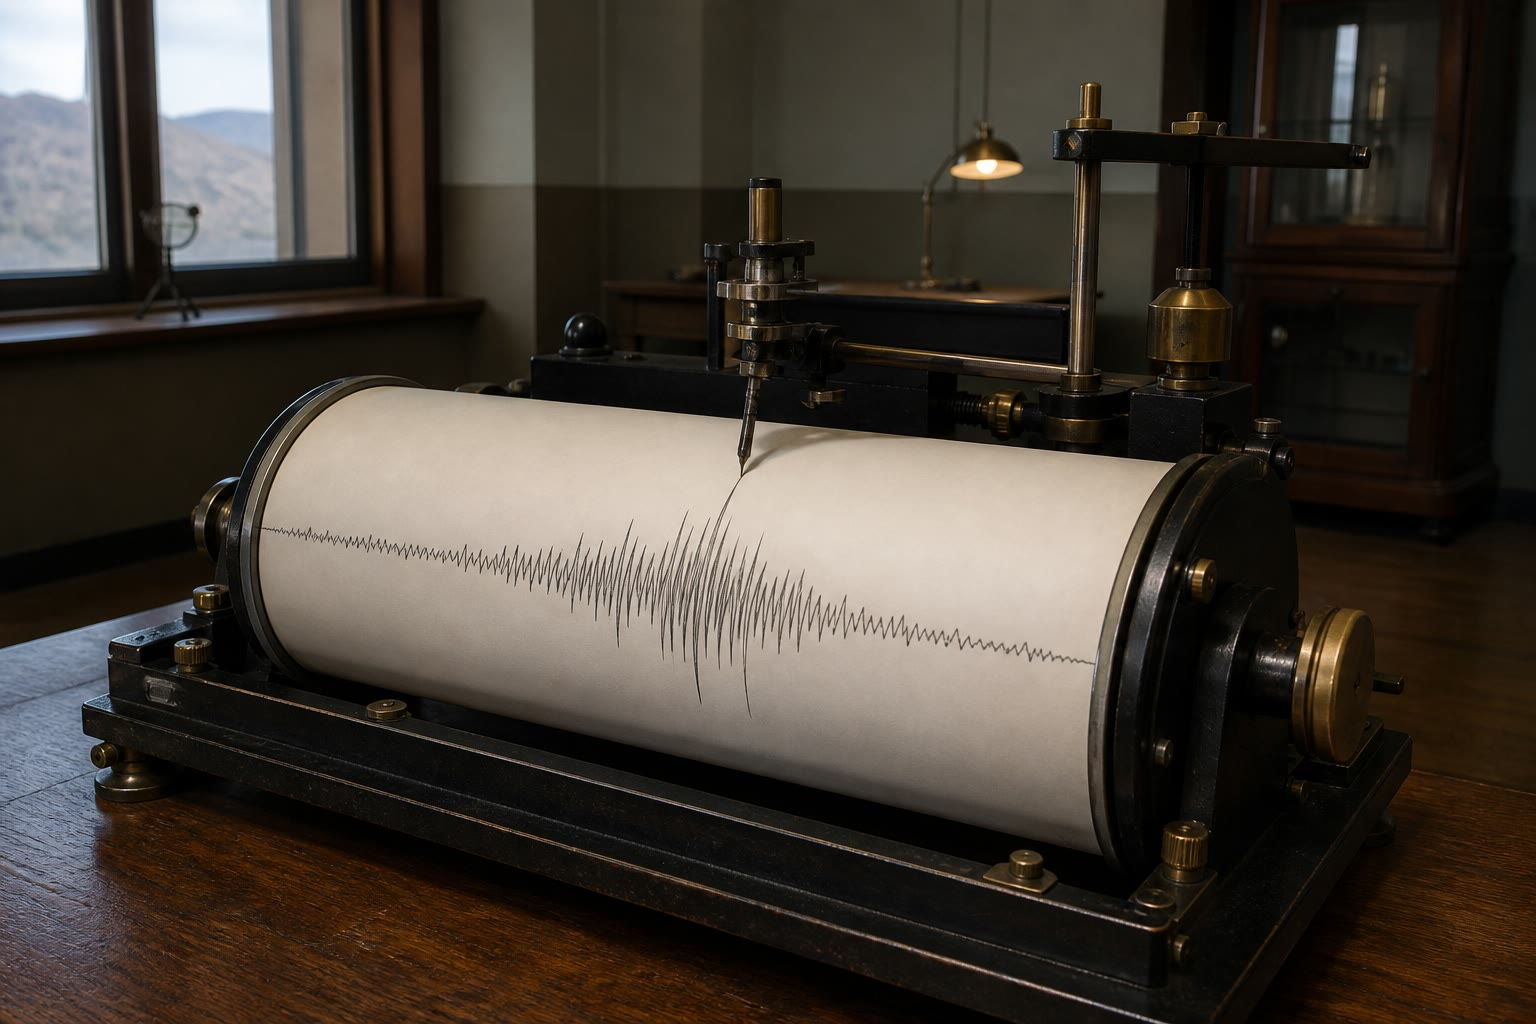
\includegraphics[width=0.58\linewidth]{images/book3/ai/b3-14-seismograph-drum.jpg}

{\small Sebuah seismograf: massa berat pada suspensi lunak tinggal diam sementara tanahnya bergerak, dan penanya menuliskan selisihnya --- osilator bereksitasi alas pada soal akhir pekan.}
\end{omfigure}

\section{Soal: Seismograf}

\begin{problem}[{Soal akhir pekan --- sebuah massa tergantung pada pegas
di dalam kotak yang dibaut ke tanah; tanahnya berguncang: apa yang
direkam penanya, mengapa alat yang sama mengukur simpangan pada
frekuensi tinggi dan percepatan pada frekuensi rendah, dan mengapa
seismometer berperiode panjang tak dapat sekadar berupa pegas panjang}]
\label{pb:b1:oscillators-resonance:1}
Sebuah massa $m = \qty{1.0}{kg}$ tergantung pada pegas berkekakuan $k$
di dalam rangka tegar yang dipasang tetap pada tanah; sebuah peredam
mengerahkan $-\alpha\dot u$, dengan $u$ simpangan massanya relatif
terhadap rangkanya, yang diukur dari kedudukan kesetimbangannya.
Tanahnya, dan karena itu rangkanya, bergerak tegak sejauh $x_g(t)$.
Kerangka bintang jauh bersifat inersial.

\medskip
\noindent\textbf{Bagian I --- Persamaannya.}
\begin{enumerate}
  \item Tuliskan kedudukan mutlak massanya sebagai $x = x_g + u +
        \text{tetapan}$, daftarkan gaya pada massanya (dalam \omterm{thm:b1:newton-dynamics:laws}{kerangka
        inersialnya}), lalu tunjukkan bahwa
        \[
        m\ddot u + \alpha\dot u + ku = -m\ddot x_g .
        \]
  \item Bawalah ke bentuk baku; kenali $\omega_0$ dan $Q$.
  \item Alatnya dibangun dengan $f_0 = \qty{0.50}{Hz}$ dan $Q = 0.70$:
        hitunglah $k$ dan $\alpha$.
  \item Percepatan tanah yang tetap $a_g$ (misalnya rangkanya
        dimiringkan) memberi $u$ tunak berapa? Tafsirkan.
  \item Apa yang direkam pena yang terpasang pada massanya, yang menulis
        pada tabung yang terpasang tetap pada rangkanya?
\end{enumerate}

\medskip
\noindent\textbf{Bagian II --- Gerak tanah yang harmonik.}
Tanahnya bergerak sebagai $x_g = X_g\cos\omega t$; tulislah $x_r = \omega/\omega_0$.
\begin{enumerate}[resume]
  \item Dengan memakai \omterm{def:b1:sinusoidal-impedance:complex}{amplitudo kompleks}, tunjukkan bahwa
        $\underline U = X_g\,x_r^2/
        (1 - x_r^2 + jx_r/Q)$.
  \item Simpulkan $U/X_g$ sebagai fungsi $x_r$ dan $Q$.
  \item Limit $x_r \gg 1$: tunjukkan $U \to X_g$ lalu jelaskan secara
        fisis apa yang dilakukan massanya (alatnya mengukur apa?).
  \item Limit $x_r \ll 1$: tunjukkan $U \approx x_r^2X_g = a_g/\omega_0^2$
        dengan $a_g$ \omterm{def:b1:wave-propagation:signal}{amplitudo} percepatan tanahnya: alatnya kini apa?
  \item Berapa nilainya pada $x_r = 1$; mengapa $Q \approx 0.7$ merupakan
        pilihan yang masuk akal?
  \item Sketsalah $U/X_g$ terhadap $x_r$ (skala logaritmik) untuk
        $Q = 0.7$ dan $Q = 5$.
  \item Berapa fase $u$ relatif terhadap $x_g$ pada frekuensi tinggi;
        tafsirkan.
\end{enumerate}

\medskip
\noindent\textbf{Bagian III --- Merancang untuk gempa bumi.}
Gempa yang jauh menghasilkan gelombang permukaan pada \qty{0.05}{}
sampai \qty{0.1}{Hz} beramplitudo milimeter; getar setempat mencapai
\qty{5}{} sampai \qty{10}{Hz}.
\begin{enumerate}[resume]
  \item Untuk merekam gelombang \qty{0.05}{Hz} sebagai simpangan orang
        menginginkan $f_0 \ll \qty{0.05}{Hz}$, katakanlah \qty{0.02}{Hz}.
        Berapa regangan statis pegasnya di bawah berat massanya? Berikan
        komentar.
  \item Sebuah \omterm{ex:b1:newton-dynamics:pendulum}{bandul sederhana} berfrekuensi sama: berapa panjangnya?
  \item Alat berperiode panjang yang sesungguhnya memakai bandul
        ``pintu pagar'' yang nyaris mendatar, atau umpan balik gaya
        elektronik. Jelaskan dalam satu kalimat apa yang dicapai
        masing-masing.
  \item Untuk alat \qty{0.50}{Hz}, hitunglah regangan statisnya: apakah
        dapat diwujudkan?
  \item Dengan alat itu, gelombang \qty{0.10}{Hz} beramplitudo
        \qty{1.0}{mm} memberi $U$ berapa? Alatnya berada dalam rezim yang mana?
  \item Getar setempat \qty{5.0}{Hz} beramplitudo \qty{1.0}{mm}: berapa
        $U$? Rezimnya?
\end{enumerate}

\medskip
\noindent\textbf{Bagian IV --- Akselerometer di dalam sebuah telepon.}
Sebuah massa hasil pemesinan mikro pada pegas silikon mempunyai
$f_0 = \qty{1.0}{kHz}$ dan $Q = 0.7$.
\begin{enumerate}[resume]
  \item Guncangan \qty{10}{Hz} beramplitudo percepatan $g$: hitunglah
        $U$. Bagaimana simpangan sekecil itu dibaca?
  \item Sampai frekuensi berapa bacaannya berada dalam $10\%$ dari
        $a_g/\omega_0^2$?
  \item \omterm{def:b1:transient-regimes:firstorder}{Tetapan waktu} $\tau = 2Q/\omega_0$ yang mana yang mengatur
        tanggapannya terhadap sebuah sentakan, dan mengapa hal itu
        berarti bagi pendeteksian sebuah jatuh?
  \item Berapa $\tau$ seismometernya: berapa nilainya dan apa akibatnya
        setelah sebuah tangga tanah yang mendadak?
  \item Mengapa peredaman kritis (atau nyaris kritis) dipilih bagi kedua
        alat itu, alih-alih $Q$ yang tinggi?
  \item Teleponnya diguncang tepat pada \qty{1.0}{kHz}: dengan faktor
        berapa bacaannya meleset?
  \item Ringkaslah: satu alat, dua rezim, yang diputuskan oleh satu
        perbandingan yang mana.
\end{enumerate}
\end{problem}
